\chapter{Opis projektnog zadatka}
		
		
		Namjera projekta riješiti je trenutačan manjak strane literature prevedene na hrvatski ili srodni jezik. Količina kvalitetne literature ograničena je i često teško dostupna u Hrvatskoj, dok web poslužitelji i stranice ne nude centralizirano rješenje za pronalazak domaćih izdanja niti jednostavnu opciju zahtjeva novih prijevoda. Naime, web stranice raznih antikvarijata nisu ažurne, metode pretraživanja nezgrapne su, a u katalogu imaju popis knjiga koji ne odgovara trenutačnom stanju u njihovim skladištima. Mnogo knjiga u njihovoj ponudi nije prevedena ili ne sadrži naslov izvornika čime je nabava željene knjige otežana.
		
		Svojim rješenjem nadamo se olakšati krajnjem korisniku pretragu i nabavku željene knjige, osobito domaćih izdanja. Naše rješenje temelji se na izradi web stranice koja služi kao posrednik između ponuditelja i korisnika, s ažurnom bazom knjiga koja brojčano nadmašuje ostale stranice. 
		
		Poseban naglasak stavljamo na literaturu prevedenu na hrvatski i jezike slične hrvatskom, a korisnicima pojednostavljujemo proces pronalaska i odabira željenog naslova dostupnošću raznovrsnih ponuditelja (izdavačkih kuća, preprodavača, antikvarijata).
		
		Web stranica služila bi kao središnje mjesto ponude različitih izdavačkih kuća, manjih knjižara i individualnih preprodavača, na taj način stvarajući veću ponudu, bolju pokrivenost i konkurentnije cijene krajnjem korisniku.
		
		Krajnjem korisniku olakšavamo pregled trenutno dostupnih knjiga na hrvatskom, srodnim i stranim jezicima. Nudimo lokacijsku preglednost ponude određenog naslova, odnosno informaciju o dostupnosti na stranom tržištu, ukoliko je knjiga nedostupna na lokalnom području.
		
		Također nudimo mogućnost zahtjeva prijevoda knjige ovisno o interesima korisnika, izdavač može ostvariti kontakt s izdavačem strane knjige i ishodovati dozvolu za prijevod knjige na jezik blizak krajnjem korisniku.\\
		
		
		
		\subsection*{Slična rješenja}
		
		Trenutno je tržište knjiga u velikoj mjeri digitalizirano. Naravno, i dalje postoje knjižare te knjige se i dalje kupuju u fizičkom obliku, ali većina izdavačkih kuća nudi svoj asortiman na web stranicama. Mnoge izdavačke kuće prenijele su dio svoje ponude na web, što je jasan pokazatelj korisničkog interesa za sličnim rješenjima.
		
		Tako, na primjer, Naklada Znanje na svom portalu nudi knjige podijeljene u kategorije knjiga prevedenih na hrvatski te strane knjige, većinom na engleskom jeziku. Njihov asortiman nije ograničen samo na knjige; imaju i kategorije poput igračaka, multimedije i slično. Na slici 2.1 vidimo njihovu web stranicu.
		
			\begin{figure}[H]
				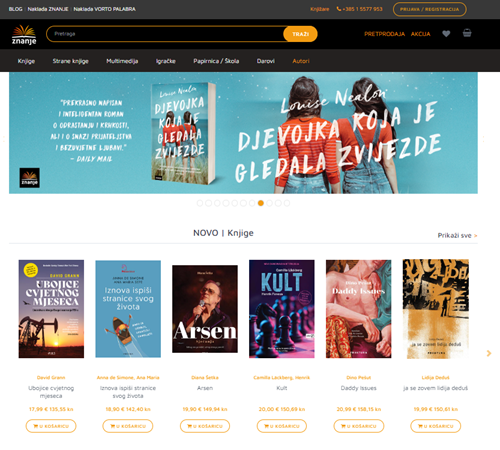
\includegraphics[scale=1]{slike/naklada-znanje.PNG} %veličina slike u odnosu na originalnu datoteku i pozicija slike
				\centering
				\caption{Web stranica naklade \textit{Znanje}}
				\label{fig:Naklada Znanje}
			\end{figure}
		
		Na njihovoj stranici možete pretraživati knjige po naslovu, autoru ili ključnim riječima, a omogućena je i jednostavna kupovina.
		
		Eknjiga.hr nudi slično rješenje, s tom razlikom da na njihovoj stranici korisnik može odabrati i izdavača u sekciji "Izdavač", omogućavajući tako izdavačima i korisnicima da lakše pristupe ponudi knjiga. Takva ponuda sliči rješenju koje mi nudimo, odnosno centraliziranom i neovisnom posredniku između ponuditelja i korisnika.
		
		Na slici 2.2 vidimo njihovo rješenje:
		
			\begin{figure}[H]
				\includegraphics[scale=1]{slike/Eknjiga.PNG} %veličina slike u odnosu na originalnu datoteku i pozicija slike
				\centering
				\caption{Web stranica \textit{Eknjiga.hr}}
				\label{fig:Eknjiga}
			\end{figure}
		
		
		Zbog sličnosti s gore navedenim, nećemo dodatno opisivati slične portale i stranice, ali ih ovdje navodimo: Mozaik knjiga, Školska knjiga, Super knjižara, Hoću knjigu, VBZ knjižara, Knjiga HR, Čitaj knjigu, Svijet knjige, Libristo, Profil knjiga, E-knjižara i mnogi drugi. Također, knjige se nude i na aplikacijama poput Njuškala.
		
		Naše rješenje razlikuje se po nekoliko aspekata. Većina postojećih platformi nudi kategorijsku podjelu knjiga, promotivne akcije i ponude usmjerene korisnicima koji ciljano pristupaju tim knjižarama kako bi pronašli određeni naslov ili se izložili širokoj ponudi te time možda pronašli knjigu od interesa. Taj pristup je usmjeren prema promociji cjelokupne ponude određenog izdavača ili nakladnika, s ciljem privlačenja korisnika na kupnju kod njih. 
		
		S druge strane, naša platforma nije posvećena jednom izdavaču, ali ne dozvoljava ni neprovjerene i privatne prodavače. Umjesto toga, dizajnirana je s korisnikom u središtu pažnje, omogućavajući mu da na temelju lokacije, jezika i naslova pronađe knjigu po najpovoljnijim uvjetima kupnje – bilo da je to cjenovna prihvatljivost, pogodna lokacija kupovine ili povjerenje u izdavača.
		
		\subsection*{Ciljna publika}
		
		Naša stranica namijenjena je svima koji žele kupiti knjigu, a osobito onima koji ne znaju strane jezike ili radije čitaju na materinjem ili srodnom jeziku. Ponuditeljima stranica nudi uvid u želje kupaca putem skupljanja zahtjeva za prijevode te platformu za prodaju.
		
		Uzimajući u obzir korisnika koji ima preferira određenog izdavača u odnosu na ostale, teško je za očekivati kako će se isti odlučiti za promjenom i našim rješenjem ukoliko odabrani naslov koji traži može pronaći kod tog izdavača.\\
		
		\noindent
		Naša web stranica namijenjena je sljedećim tipovima kupaca:
		
		\begin{packed_enum}
			\item korisniku sa specifičnim zahtjevom knjige na preferiranom jeziku ili određenoj lokaciji, kojemu je u interesu pronaći knjigu koju možebitno nema u katalogu izdavača od povjerenja
			\item korisniku koji po lokaciji i odabranom jeziku želi pregledati ponudu knjiga koje bi ga mogle zanimati
			\item neodlučnom korisniku koji nije siguran u odabir knjige (cijena, udaljenost izdavača)
		\end{packed_enum}
		
		\noindent
		Registriranim ponuditeljima naša stranica nudi:	
		
		\begin{packed_enum}
			\item stranicu sa značajkama atraktivnim kupcima
			\item izbjegavanje potrebe vlastitog web rješenja
			\item mogućnošću prodaje knjiga koje su rijetko kupovane te su ispale iz glavne ponude
			\item uvid u želje korisnika za prijevodima
		\end{packed_enum}
		
		\subsection*{Opseg implementacije}
		
		Projektni zadatak ima za cilj izvesti web aplikaciju prilagođenu mobilnom uređaju ili tabletu.
		
		Korisnici se dijele na neregistrirane i registrirane, što povlači izvedbu procesa registracije u aplikaciju koja će se odvijati uz pomoć spremanja korisničkog imena i lozinke u bazu podataka. Prilikom registracije, korisnik je dužan navesti podatke koji će biti vidljivi na njegovom profilu unutar aplikacije: naziv, e-pošta, adresa, broj telefona.
		
		Provjeru valjanosti registracije obavlja administrator po registraciji korisnika.
		Registrirani korisnik dijeli se na tri vrste: izdavač, antikvarijat te preprodavač.
		Neregistrirani korisnik ima pristup ponudi knjiga i  pretrazi kataloga knjiga (svih dostupnih knjiga na aplikaciji). Pretraga kataloga knjiga omogućena je prema značajkama knjige (naslovu, autoru), nazivu ponuditelja (naziv registriranog korisnika, neovisno o kategoriji) te prema lokaciji ponude. 
		
		Pretraživanje knjige za rezultat ima listu ponudu za istu koja sadrži naziv ponuditelja, broj dostupnih	primjeraka i cijenu knjige kod dotičnog ponuditelja, ukoliko isti zapisi postoje u bazi registriranih korisnika. Neće se prikazivati one knjige  za koje nema zapisa u bazi podataka  ili nije označena kao dostupna i kod jednog  korisnika.
		
		Lokacija ponude bit će izvedena preko interaktivne karte na kojoj će biti označeni registrirani ponuditelji koji u svojoj ponudi imaju aktivan i ažuriran asortiman knjiga. Krajnjem korisniku omogućen je pregled svih adresa  (lokacija) ponuditelja te odabir pojedinog ponuditelja. Odabir ponuditelja vrši se klikom na ikonicu ponuditelja označenoj na mapi, nakon čega se izlistava asortiman knjiga istog ponuditelja.
		
		Projekt predviđa i rješenje baze podataka u koju se spremaju podaci registriranih korisnika i podaci o knjigama.
		
		Korisnički podaci su korisničko ime, lozinka, naziv korisnika,  e-pošta, adresa, broj telefona.
		
		Podaci o knjigama su: naziv, autor, godina izdanja, izdavač, kategorija izdavača (domaći, strani), žanr, ISBN, broj izdanja, stanje očuvanosti, opis, slika korica, oznaka vrste knjige te dostupnost.
		
		Rješenje isto tako predviđa i da neregistrirani korisnici imaju mogućnosti  kroz sučelje aplikacije zatražiti od izdavača da kontaktira stranog izdavača oko prijevoda strane knjige na hrvatski jezik. 
		